%%%%%%%%%%%%%%%%%%%%%%%%%%%%%%%%%%%%%%%%%%%%%%%%%%%%%%%%%%%%%%%%%%%%%%%%%%%%%%%%%
% Macros
%%%%%%%%%%%%%%%%%%%%%%%%%%%%%%%%%%%%%%%%%%%%%%%%%%%%%%%%%%%%%%%%%%%%%%%%%%%%%%%%%
\documentclass[conference]{IEEEtran}
\IEEEoverridecommandlockouts
% The preceding line is only needed to identify funding in the first footnote. If that is unneeded, please comment it out.
\usepackage{cite}
\usepackage{amsmath,amssymb,amsfonts}
%\usepackage{algorithmic}
\usepackage{graphicx}
\usepackage{textcomp}
\usepackage{xcolor}

\usepackage{preamble}

\usepackage{pifont} % Check and cross marks

\begin{document}

    \title{Fast and Easy Affective Computing on Multi-Core Wearable Devices}

    \author{
        \IEEEauthorblockN{\yiltan}
        \IEEEauthorblockA{
            ECE Department \\
            Queen's University \\
            Kingston, Canada \\
            yiltan.temucin@queensu.ca
            }
        \and
        \IEEEauthorblockN{Amir Hossein Sojoodi}
        \IEEEauthorblockA{
            ECE Department \\
            Queen's University \\
            Kingston, Canada \\
            amir.sojoodi@queensu.ca
            }
        }

    \maketitle

    \begin{abstract}
        Abstract

    \end{abstract}

    \begin{IEEEkeywords}
        Affective Computing, Machine Learning, ELEC872
    \end{IEEEkeywords}

    \section{Introduction}

    \section{Background}
\label{sec:background}
\subsection{Sensors}
Affective computing often relies on gathering data from human sources.
Many different types of sensors exist for
gathering information which can be important in this area.
In this paper we will focus on the following three types of sensors;
Electrocardiography,
Electroencephalography,
and Galvanic Skin Response.

\subsubsection{Electrocardiography (ECG)}
Sensors are used to measure muscle activity.
As muscles contract and relax,
electrical signals are sent via neurons.
These electrical signals then
can be recorded using various types of sensors.
One of the main types of sensors is sEMGs;
they are usually placed on the belly of the muscle
and are cleaned with alcohol before placing
on the surface of the skin.
These sensors can be used to measure
the PQRST complex of a heartbeat.
Each part of the PQRST complex
corresponds to a part of the heart's cycle as it pumps blood around the body.

\subsubsection{Electroencephalography (EEG)}
EEG is a method to record brain activity.
They measure the electrical signals which the brain generates.
As neurons in the brains send information,
electrical currents are generated and are then measured.
This procedure is difficult to setup,
an amount gel is placed onto the scalp, then sensors are placed upon them.
Many different frequency bands can be filtered from these
signals to obtain different information about brain activity.

\subsubsection{Galvanic Skin Response (GSR)}
GSR is placed directly onto the skin of the participants.
The state of a sweat gland varies the resistance of human skin.
Studies have shown that sweating is controlled by the sympathetic nervous system
therefore we can collect this information
to build models on the system's behaviour.

\subsection{Amigos Data set}
The AMIGOS data set was prepared by research groups at
Queen Mary University of London, United Kingdom and
University of Trento, Italy \cite{AMIGOS:2018}.
This data set allows for research to be conducted on
personality traits, mood and affect.

The data set contains 40 participants who each watched 20 videos.
These 20 videos are split into two categories; long and short.
Each of these categories is first split into
whether the participant watched the video alone or within a group.
Data was collected using ECG, EEG, and GSR sensors.
The participants were also recorded, but we will not use the video recordings
for our work.
These videos were labelled with:
valence, arousal, control, familiarity, like/dislike,
and selection of basic emotions.

\subsection{Machine Learning}
Machine Learning (ML) uses statistical models and
optimisation algorithms to model a problem.
ML often requires large volumes of data to generalise a problem.
Representation Learning is when the original data is not learned
but rather transferred into a different form in which is learned.
One example would be using feature extraction.
Features are extracted from data sets and then this new representation of the data
is learned.
Another common problem is having too much data which causes slow training times.
Techniques like dimension reduction are used to reduce the volume of
data.

Many different models are used to classify data within machine learning,
some of the most popular are SVM, KNN, Naive Bayes.
SVMs try to fit a plane between many data points.
This algorithm often has problems with data which is not
linearly separable.
KNN algorithm finds the K-nearest neighbours to each data point.
This algorithm is simple to implement but it does not scale well
to large data sets as the distance between any two points must be calculated.
The Naive Bayes is also another simple model which is used but the main issue
with using this that it makes an assumption about the underlying distribution of
our data.

\subsection{Motivation}
The new AMIGOS data set has provided researchers with new
data which has not been previously collected.
Using signals such as ECG, EEG, and GSR
could we create a mapping to the
labels of the videos such as
valence, arousal, control, familiarity, like/dislike,
and selection of basic emotions?
Other existing work has focused on using a single signal types
(some have studied multiple of the same type) from this data set
and they did not incorporate any multi-processing.


    \section{Related Work}
\label{sec:related_work}
In \cite{sarkar2020selfsupervised} Sarkar and Etemad
used the EEG signals from the AMIGOS data set to classify emotions.
They used a signal transformation recognition networks
where they learned representations of unlabelled EEG signals.
These weights were then transferred to a pre-existing emotional
recognition framework.
Although there model performed better than some state of the art models
they had issues with subject independent emotion recognition.

Harper and Southern used the ECG signals from the AMIGOS data set
and fed this data into a Bayesian framework to model
the uncertainty of the valence predictions \cite{Harper_2020}.
They also compared made comparisons to LSTM and CNN models with
and without their Bayesian framework.
This approach with did not account for multi-modal input.

The Deep Belief-Conditional Random Field Framework was used by
Chao and Lui in \cite{8999626}.
In this work they used the many different EEG channels as inputs to their system.
They trained each channel independently and use ensemble methods to combine the outputs.
Using this method they were not able to outperforms other state of the art methods
but they did show that this method is comparable and domes have promise.

In \cite{LI2020102185} Li et. al used LSTMs.
This avoided manual labour of designing and extracting features.
Before feeding the data into the LSTM they transformed the signals into spectrograms.
Their methods is also multi-model and incorporates many different signals which
are present in the AMIGOs datset.
Using this method they were able to detect emotions from the raw signals and outperform some of the current best works in this area.


Martínez-Tejada et. al showed that age, sex, personality type did not
correlate with the detection of emotion, arousal or valiane when using
machine learning algorithms \cite{Mart_nez_Tejada_2020}.
They used relatively simple algorithms to the other works discussed.
They use SVMs, Naive Bayes, and random forests for their tests.
These tests were carried out independently from one another.
In their discussing they did comment on whether the use of these
samples models where the reason behind not finding a strong correlation
or whether there was not a correlation to begin with.

The work by Yang and Lee in \cite{8683290}  developed
a attribute-invariance loss embedded variational autoencoder (AI-VAE).
When compared to traditional variational autoencoders (VAE)
they saw that they were able to achieve a 6.5\% performance improvement.

All of these works do not use all of the various signals offered by the AMIGOS data set.
The goal of our work is to combine all of the EEG, ECG, and GSR signals for our feature extraction phase.
We want so see if combining different signals from the same video sample
allows us to better classifier our problem.


    \section{Proposed Method}
\label{sec:proposed_method}
\begin{figure}[b]
    \centering
    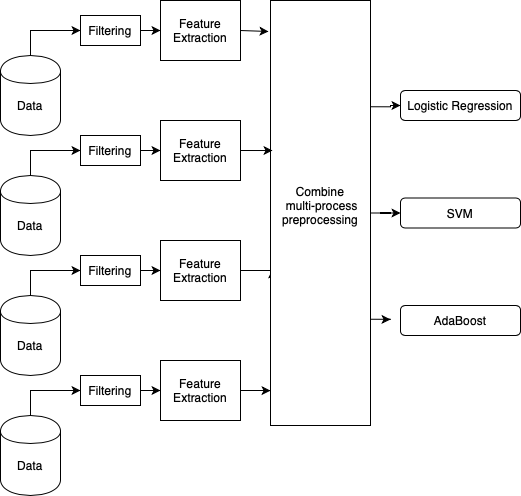
\includegraphics[width=\columnwidth]{tex/figures/model.png}
    \caption{Our Proposed Method}
    \label{fig:model}
\end{figure}

Our preliminary testing found that reading and the preprocessing stage
was very slow.
To combat this we designed a multi-processes preprocessing stage.
Here each process reads a chunk of the data and applies filtering,
feature extraction, and dimensional reduction independently.

For filtering we use a butter worth filter with various cutoffs which are dependent on the signal in which we are processing.
Band notch is used to remove power line hum and high pass filters are used to remove
baseline wander.
For feature creation we split the EEG signal into its alpha, beta, theta, and gamma bands.
From this we created the features by splitting the power from each band

For dimensional reduction we reduced the 368 dimensions using PCA
and then selecting the top 40 vectors.
Although this is a significant reduction in dimension we keep 82\% of our
original variance.

Then these processes join and are fed into 3 different classifiers;
A Logistic Regression, SVM, and KNN.
We also tried to use Naive Bayes but we were unable to get it working.
These classifiers are independent and the output of each is measured.
We also feed each output into a voting classifier.
If we had time we would have continued our multiprocessing efforts to do each
classification in parallel to further reduce run time.

    \section{Experimental Results}
\label{sec:experimental_results}
\subsection{Software Platform}
For our tests we are using \texttt{pandas},
a data manpilation librirary,
for reading data in structured formats such as
\texttt{.csv} and \texttt{.xlxs} files.
The AMIGOS dataset is avaible in \texttt{.mat} format.
As we would like to use Python for our work we used
the library \texttt{SciPi} to read this format in a Python friendly manner.
This library was also used for the signal processing portion of our project.
For ploting of figures we used \texttt{matplotlib.pyplot}.
For the various algorithms we used throughout this paper such as SVM we
used \texttt{sklearn}.
\begin{figure}[h]
    \centering
    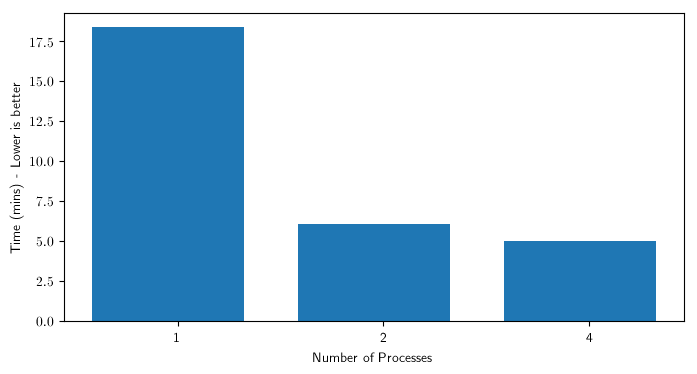
\includegraphics[width=\columnwidth]{tex/figures/multiprocess/multi_process_time.png}
    \caption{Time Taking to pre process data for different number of processes.}
    \label{fig:multip:time}
\end{figure}


\subsection{Performance of Multi-Process Feature Extraction}
On a 4 core Intel i5 processes we tested the performance of our feature extraction
for 1, 2, and 4 processes.
In Figure \ref{fig:multip:time} we can see the time taken to read and process
the data for these different process counts.
For a single process it took over 18 minuits to extract features.
There is only a minuit difference between the 2 and 4 process feature extraction phase.
That said we were able to get our time down to under 5mins.
This is around 3.6x improvemtn in performance.
While this does not improve our classification, this allowed us play
with our hyper parameters more frequently as each test took less time.
\begin{figure*}[h]
    \centering
    \begin{subfigure}[t]{\columnwidth}
        \centering
        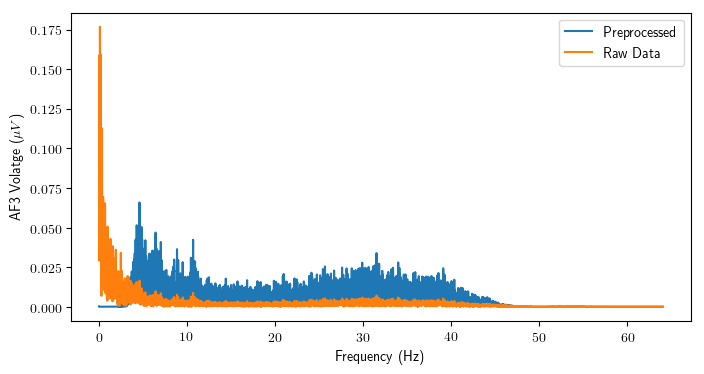
\includegraphics[width=\columnwidth]{tex/figures/filtering/AF3.png}
        \caption{AF3}
        \label{fig:filter:af3}
    \end{subfigure}
    \hfill
    \begin{subfigure}[t]{\columnwidth}
        \centering
        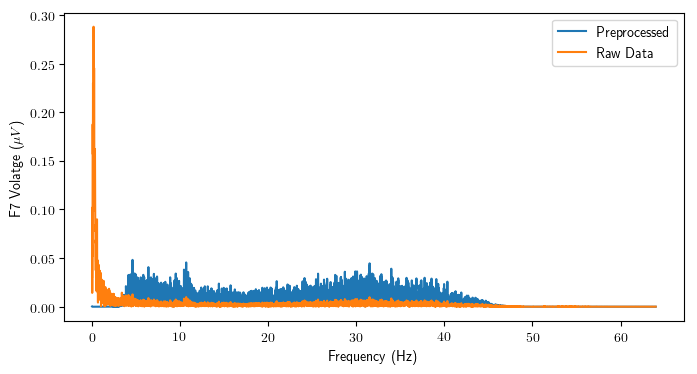
\includegraphics[width=\columnwidth]{tex/figures/filtering/F7.png}
        \caption{F7}
        \label{fig:filter:f7}
    \end{subfigure}
    \caption{Example filtering of EEG signal on sample 1 video 12}
    \label{fig:eeg}


    \begin{subfigure}[t]{\columnwidth}
        \centering
        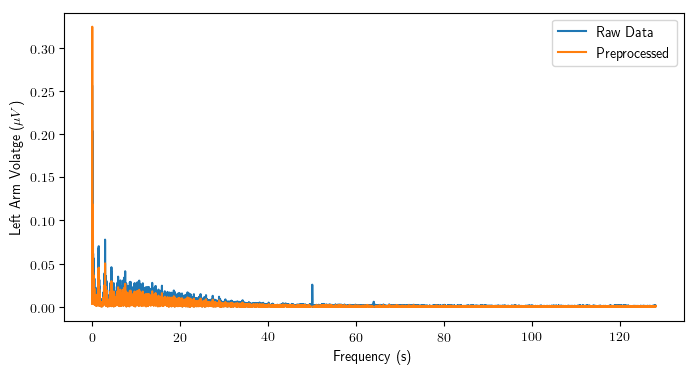
\includegraphics[width=\columnwidth]{tex/figures/filtering/ECG Left Arm.png}
        \caption{Left}
        \label{fig:filter:left}
    \end{subfigure}
    \hfill
    \begin{subfigure}[t]{\columnwidth}
        \centering
        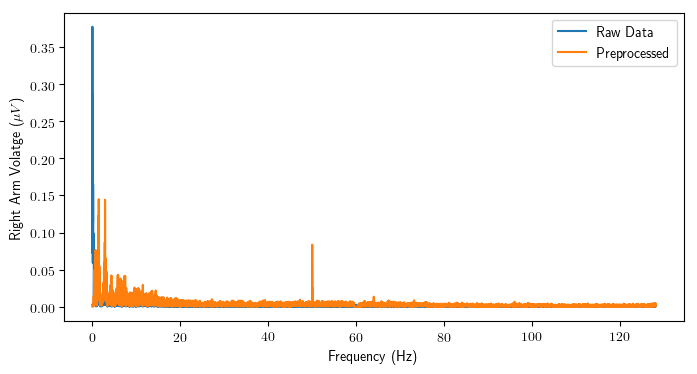
\includegraphics[width=\columnwidth]{tex/figures/filtering/ECG Right Arm.png}
        \caption{Right}
        \label{fig:filter:right}
    \end{subfigure}
    \caption{Example filtering of ECG signal on sample 1 video 12
             for the left and right arms}
    \label{fig:ecg}
\end{figure*}


\subsection{Preprocessing}
We have applied 3 processing steps to our AMIGOS dataset;
signal filtering, feature extraction, and dimentionality reduction.
In Figures \ref{fig:eeg} and \ref{fig:ecg}
we can see our filters applied to the EEG and ECG signals in the frequency domain.
For the EEG signal we followed the guideline set on the AMIGOS
website and applied a 4-45Hz bandpass filter \cite{AMIGOS:2018}.
We removed a significant amount of low frequency noise.
We can see that the preproccessed data results
in an slightly high amplitude than our original signal despite keeping the same shape.
Through experimental analysis we noticed that this was by a factor of 5.
For the ECG signal we applied a 0.05Hz highpass filter as noted in
\cite{SantamariaGranados:2019}
to remove baseline wander.
We also applied a bandstop filter with a 50Hz cutoff.
A small notch is visible in
Figures \ref{fig:ecg}.
The impact of the frequency filtering in the time domain can be seen in Figure
\label{fig:ecg:time}.

\subsection{Classification Results}
\begin{table}[h]
\caption{Logistic Regression}
\label{table:logistic}
\centering
\begin{tabular}{|c|c|c|}
\hline
\textbf{Emotion} &  \textbf{F1} &  \textbf{Accuracy} \\ \hline \hline
neutral & 0.685 & 0.713 \\ \hline
disgust & 0.889 & 0.900 \\ \hline
happiness & 0.858 & 0.8875 \\ \hline
surprise & 0.788 & 0.813 \\ \hline
anger & 0.487 & 0.538 \\ \hline
fear & 0.756 & 0.800 \\ \hline
sadness & 0.720 & 0.738 \\ \hline
\end{tabular}
\end{table}
\begin{table}[h]
\caption{SVM}
\label{table:svm}
\centering
\begin{tabular}{|c|c|c|}
\hline
\textbf{Emotion} &  \textbf{F1} &  \textbf{Accuracy} \\ \hline \hline
neutral& 0.678 & 0.713  \\ \hline
disgust& 0.889 & 0.900 \\ \hline
happiness& 0.871 & 0.913 \\ \hline
surprise& 0.811& 0.850 \\ \hline
anger& 0.457& 0.525 \\ \hline
fear& 0.775 & 0.838 \\ \hline
sadness& 0.747 & 0.763 \\ \hline
\end{tabular}
\end{table}
\begin{table}[h]
\caption{KNN}
\label{table:knn}
\centering
    \begin{tabular}{|c|c|c|c|}
\hline
\textbf{Emotion} &  \textbf{F1} &  \textbf{Accuracy} & \textbf{Best K}\\ \hline \hline
neutral& 0.712& 0.725& 5 \\ \hline
disgust& 0.916& 0.925& 2 \\ \hline
happiness& 0.871& 0.9125& 4 \\ \hline
surprise& 0.827& 0.875& 16 \\ \hline
anger& 0.559& 0.575& 1 \\ \hline
fear& 0.794& 0.8375& 4 \\ \hline
sadness& 0.864& 0.875& 2 \\ \hline
\end{tabular}
\end{table}
\begin{table}[h]
\caption{AdaBoost}
\label{table:adaboost}
\centering
    \begin{tabular}{|c|c|c|}
\hline
\textbf{Emotion} &  \textbf{F1} &  \textbf{Accuracy} \\ \hline \hline
neutral& 0.683& 0.688 \\ \hline
disgust& 0.901& 0.925 \\ \hline
happiness& 0.852& 0.875 \\ \hline
surprise& 0.875& 0.875 \\ \hline
anger& 0.718& 0.725 \\ \hline
fear& 0.782& 0.775 \\ \hline
sadness& 0.785& 0.788 \\ \hline
\end{tabular}
\end{table}
\begin{table}[h]
\caption{Voting}
\label{table:voting}
\centering
    \begin{tabular}{|c|c|c|}
\hline
\textbf{Emotion} &  \textbf{F1} &  \textbf{Accuracy} \\ \hline \hline
neutral& 0.685& 0.713 \\ \hline
disgust& 0.895& 0.913 \\ \hline
happiness& 0.871& 0.913 \\ \hline
surprise& 0.811& 0.850 \\ \hline
anger& 0.660& 0.688 \\ \hline
fear& 0.775& 0.838 \\ \hline
sadness& 0.842& 0.863 \\ \hline
\end{tabular}
\end{table}

In Tables \ref{table:logistic}, \ref{table:svm}, \ref{table:knn}, and \ref{table:voting}
we have the output of the different classification methods which we used.
With all three methods we that the F1 scores and the accuracy are very close.
The exact accuracy which we obtain differs between the emototions which we try and classify.
That said generally the KNN results are better than the SVM and the Logistic Regression.
This could be because its a better model or because it is over fitting.
To be certain of KNN's superiour classification.


    \section{Conclusion}
\label{sec:conclusion}
From our work we have seen that using multiple processes
for data parallellis within our machine learning model allows for significant imrpovements in the time take to run the program.
Unfortunatly this does not improve the classification performance.
The 3 different classifies Logistic Regression,
SVM, and KNN
all have the befifits and disadvantages.
We would suggests that users should use the model that more accuratly detects
the emotion that they are interested in if there were to use our code.
One possible extension to our work would be to use ensamble methods to
combine the outputs of each of our classifiers.
This would improve our overall performance.


    \section{Division of Work}
\label{sec:division_of_work}
Git commit history of attached project and
\LaTeX~files should show the distribution.
A summery is bellow.

\subsection{Yiltan}
Yiltan setup the \LaTeX~and Python Projects.
Created the reader functions related to parsing the Excel data.
Wrote the Python code for pre-processing of the AMIGOS data
and the related section in the paper.
Yiltan also wrote the introduction, background, and related works
sections of this paper.
[TODO]

\subsection{Amir}
Amir prepared and downloaded the Amigos dataset.
He also developed the reader for parsing the dataset
which was in matlab format.
Amir also worked on the piece of code that involved reducing the dimention of our data.
[TODO]


    \bibliographystyle{IEEEtran}
    \bibliography{cite}

    \clearpage
\onecolumn
\appendix
\begin{appendices}
  \section{Source Code}
  \noindent
  Source code has also been attached to this submission
  but they are attached here for ease of marking.

  \subsection{Reader}
  \noindent
  This code is used to read the AMIGOS data set.
  \lstinputlisting[language=Python]{src/reader.py}

  \subsection{Reader}
  \noindent
  This code defines the high/low/band-pass filters
  which are used in our work.
  \lstinputlisting[language=Python]{src/filters.py}

  \subsection{Prepossessing}
  \noindent
  This file contains the Prepossessing of our data.
  It relies on the previous filtering code.
  \lstinputlisting[language=Python]{src/preprocess.py}

  \subsection{Dimension Reduction}
  \noindent
  This file contains code for the dimension reduction portion of our model.
  \lstinputlisting[language=Python]{src/dimension_reduction.py}

  \subsection{Machine Learning Algorithms}
  \noindent
  This file contains code for the machine learning algorithms portion of our model.
  \lstinputlisting[language=Python]{src/learning.py}

  \subsection{Benchmarking The Multiprocessing}
  \noindent
  This file contains code for the the benchmarking of 1-4 processes.
  \lstinputlisting[language=Python]{src/bench_preprocess.sh}

  \subsection{Plotting}
  \noindent
  This is the for the plotting of our figures used in this paper.
  \lstinputlisting[language=Python]{src/plot.py}

\end{appendices}


\end{document}
\endinput
